% LTeX: language=de-DE

\chapter{Umsetzung}

Im Folgenden wird die Umsetzung einer Integration eines Security Keys in Kombination mit \ac{FIDO}2 innerhalb der \ac{LSY} beschrieben. Dabei wird der aktuelle Stand berücksichtigt und begründet ein passender Ansatz für die Integration gewählt. Zusätzlich wird die Umsetzung zum Aspekt der Benutzerfreundlichkeit analysiert.

\section{Aktueller Stand der LSY} \label{current}
Innerhalb der \ac{LSY} werden aktuell verschiedene Verfahren zur Authentifizierung genutzt. Grundsätzlich besteht eine zentrale Nutzerverwaltung innerhalb der \ac{LSY}, welche innerhalb einer Microsoft Azure \ac{AD} verwaltet wird. Wie diese an eine Applikation gebunden ist, ist dabei nicht vorgegeben und kann von den jeweiligen ABteilungen individuell festgelegt werden. Auch Lösungsansätze ohne die Nutzung der Azure \ac{AD} sind je nach Abteilung möglich. Die einzige zentrale Schnittstelle ist somit die genannte Azure \ac{AD}.

Diese bestehende Nutzerverwaltung basiert auf einer passwortbasierten Authentifizierung inklusive \ac{MFA}. Das Passwort muss von allen Nutzern in regelmäßigen Abständen (drei Monate) geändert werden. Der weitere Faktor für die Nutzung der \ac{MFA} kann frei von den Nutzern gewählt werden, solange er mit der Azure \ac{AD} kompatibel ist. Zusätzlich zur regelmäßigen Passwortänderungen, gibt es Richtlinien zur Passworterstellung, welche von den Nutzern eingehalten werden müssen. 

Grundsätzlich ist eine Integration eines Security Keys als \ac{SFA} mit Hilfe einer Azure \ac{AD} möglich. Diese Funktion ist innerhalb der \ac{LSY} allerdings nicht aktiviert, da diese Art der Authentifizierung nicht den Richtlinien des Unternehmens entspricht. Eine Änderung dieser Richtlinien ist möglich, erfordert allerdings einen sehr hohen Aufwand und viel Zeit. Lediglich die Verwendung eines Security Keys als zweiten Faktor für eine \ac{MFA} wird von der \ac{LSY} unterstützt und ist auch mit der Azure \ac{AD} kompatibel (siehe \textbf{\ref{azure-seckey}}) Da der Bearbeitungsraum dieser Arbeit zeitlich limitiert ist, wird aus den genannten Gründen keine \ac{LSY} weite Integration eines Security Keys betrachtet. Dennoch soll eine Integration in einem kleinerem Rahmen auf Abteilungsebene getestet werden. Dies soll eine Aussage ermöglichen, ob eine Umstellung der aktuellen Richtlinien sinnvoll ist und eine Integration eines Security Keys in der gesamten \ac{LSY} möglich ist.

\begin{figure}[h]
	\centering 
	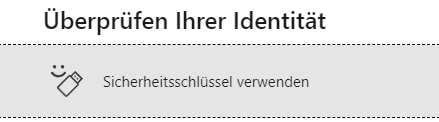
\includegraphics[width=0.6\textwidth]{img/abbildungen/azure_seckey.png}
	\captionsetup{format=hang}
	\caption{Security Key als zweiter Faktor in der Azure \ac{AD}} \label{azure-seckey}
\end{figure}

Für diese Testphase wird die Abteilung cGroup Solutions ausgewählt. Diese ist zuständig für das Produkt cFront, welches in \textbf{\ref{cFront-exp}} beschrieben ist. Innerhalb der Abteilung wird aktuell eine passwortbasierte Authentifizierung gegen die Azure \ac{AD} inklusive \ac{MFA} genutzt. Vorteilhaft für die Integration eines Security Keys ist, dass die Abteilung zusätzlich Keycloak für die Identitäts- und Zugriffsverwaltung nutzt. Keycloak ist eine Open-Source-Plattform für Identitäts- und Zugriffsmanagement, die Single Sign-On, Benutzerverwaltung und Sicherheitsfunktionen bietet, um die Authentifizierung und Autorisierung in Anwendungen zu erleichtern. Es wird verwendet, um Benutzer sicher anzumelden, ihre Zugriffsrechte zu verwalten und die Integration mit anderen Identitätsdiensten zu unterstützen \cite{keycloak}. Somit bietet sich eine neue Schnittstelle für die testweise Integration eines Security Keys an, da Keycloak zwar die Schnittstelle zur Azure \ac{AD} nutzt, allerdings zusätzlich auch eine eigene Nutzerverwaltung besitzt. Dies erfordert keine Änderungen der aktuellen Richtlinien oder große technische Umstellungen innerhalb der gesamten \ac{LSY}, sondern ermöglicht eine Integration auf Abteilungsebene.

Die aktuelle Umsetzung der Abteilung zur Authentifizierung ist vereinfacht in \textbf{\ref{current-imp}} abgebildet. Die Applikation kommuniziert nicht direkt mit dem Keycloak-Server, sondern nutzt eine selbst entwickelte Anwendung, welche sich als Keycloak-Client ausgibt. Der Nutzer gibt seine Zugangsdaten bei der Anmeldung an den Keykloak-Client weiter. Dieser wandelt die Zugangsdaten in einen validen JWT-Token um und übergibt diesen an den Keycloak-Server. Der Keycloak-Server validiert die Zugangsdaten gegen die Azure \ac{AD} und authentifiziert den Nutzer, indem er einen oAuth2-Token erstellt und diesen an die Applikation zurückgibt.


\begin{figure}[h]
	\centering 
	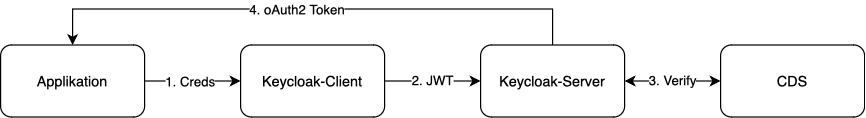
\includegraphics[width=1\textwidth]{img/abbildungen/Unknown.png}
	\captionsetup{format=hang}
	\caption{Aktuelle Umsetzung der Abteilung} \label{current-imp}
\end{figure}

\section{Wahl des Security Keys} \label{secwahl}
Für die Umsetzung der passwortlosen Authentifizierung innerhalb der \ac{LSY} wurde ein Yubikey der Series 5 mit NFC gewählt. Dieser wurde in Kapitel vorgestellt. Hingewiesen sei an dieser Stelle, dass auch andere Hersteller Security Keys anbieten, welche das FIDO2-Protokoll unterstützen. 

Dazu gehören unter anderem:
\begin{itemize}
    \item \textit{Feitian ePass} des Herstellers FEITIAN Technologies Co., Ltd.
    \item \textit{Titan} des Herstellers Google
    \item \textit{SafeNet eToken} des Herstellers Thales Group
\end{itemize}

Die Wahl des Security Keys richtete sich allerdings unter anderem an der Kompatibilitätsliste \cite{compWin} von Microsoft. Diese listet alle Security Keys auf, welche für eine passwortlose Authentifizierung gegen eine Microsoft Azure \ac{AD} genutzt werden können. Nicht auffindbar in der Liste ist beispielsweise der Google Titan. Dieser unterstützt aktuell nicht FIDO2, sondern lediglich FIDO und \ac{U2F}. Microsoft ist allerdings nicht abwärtskompatibel, was bedeutet, dass der Google Titan nicht für eine passwortlose Authentifizierung gegen das Azure \ac{AD} genutzt werden kann .

Die endgültige Auswahl basiert auf dem bestehenden Bestand eines Yubikeys der Series 5 mit NFC. Dieser ist mit der Azure \ac{AD} nutzbar. Grundsätzlich ist allerdings auch eine Nutzung eines anderen Security Keys möglich, sofern dieser das \ac{FIDO}2-Protokoll unterstützt, in der Kompatibilitätsliste von Microsoft aufgeführt ist und und offiziel von der \ac{FIDO} Allianz zertifiziert wurde.

Sollte die Nutzung eines Security Keys innerhalb der \ac{LSY} in Zukunft erweitert werden, so wird eine neue weitreichende Analyse notwendig. Da im Rahmen dieser Arbeit lediglich eine Testphase auf Abteilungsebene stattfindet und die grundsätzliche Funktionsweise der unterschiedlichen Security Keys ähnlich ist, wird auf eine detaillierte Analyse der unterschiedlichen Security Keys verzichtet.

\section{Integration eines Yubikeys in die LSY}

Grundsätzlich bieten sich zwei Möglichkeiten für die Integration eines Security Keys in die Abteilung cGroup Solutions an. Die erste Option wurde bereits \textbf{\ref{current}} beschrieben. Hierbei würde eine Authentifizierung der Nutzer ohne Umwege gegen die Azure \ac{AD} stattfinden, wie in \textbf{\ref{azure-imp}} vereinfacht dargestellt. Diese Option ist nativ mit der Azure \ac{AD} kompatibel und erfordert technisch lediglich eine Anpassung der aktuellen Konfiguration. Dies würde zu einer \ac{LSY} weiten Integration führen, da die Azure \ac{AD} als zentrale Nutzerverwaltung genutzt wird.

\begin{figure}[h]
	\centering 
	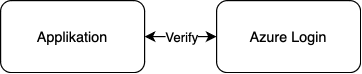
\includegraphics[width=0.6\textwidth]{img/abbildungen/azure_umsetzung.png}
	\captionsetup{format=hang}
	\caption{Umsetzungsmöglichkeit mit Azure \ac{AD}} \label{azure-imp}
\end{figure}

Die zweite Option würde Gebrauch von der Schnittstelle des Keycloak-Servers innerhalb der Abteilung cGroup Solutions zu machen. Diese Option würde somit nur die Abteilung betreffen und erfordert eine technische Veränderung der aktuellen Konfiguration des Keycloak-Servers. Hierbei würden nur bestimmten Nutzern die Möglichkeit gegeben werden, sich mit Hilfe eines Security Keys anzumelden, da der Security Key lediglich vom Keycloak-Server dem Nutzer zugeordnet wird. Also hat diese Option keine Auswirkungen auf die zentrale Nutzerverwaltung. 

Da es sich wie in \textbf{\ref{current}} beschrieben lediglich um eine Testphase handelt, welche nur die Abteilung cGroup Solutions betrifft, wird die zweite Option gewählt. Dies liegt insbesondere an dem hohen organisatorischen Aufwand die aktuellen Richtlinien der \ac{LSY} verändern zu lassen und die technische Umstellung der Azure \ac{AD} zu beantragen. Da die zentrale Nutzerverwaltung ein wichtiger Bestandteil aller Applikationen ist, wäre zudem ein zu hohes Risiko vorhanden, sollten technische Probleme auftreten. 

Um die genannte Option mit Hilfe von Keycloak umzusetzen, müsste der aktuelle Prozess aus \textbf{\ref{current-imp}} wie folgt angepasst werden:

\begin{figure}[H]
	\centering 
	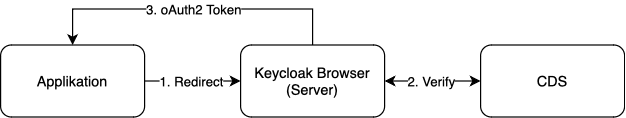
\includegraphics[width=1\textwidth]{img/abbildungen/keycloak_browser.png}
	\captionsetup{format=hang}
	\caption{Veränderter Keycloak-Login}
\end{figure}

Statt die Anmeldung eines Client zu simulieren, lässt sich mit  Keycloak eine Anmeldung über eine Nutzeroberfläche realisieren. Diese wird dabei selbst von Keycloak gestellt. Dafür wird ein redirect auf die Keycloak Login-Seite durchgeführt. Bei einer erfolgreichen Verifizierung wird der Nutzer zurück auf die Applikation geleitet und vom Keycloak-Server mit Hilfe eines oAuth2-Tokens authentifiziert. 

Diese Umstellung muss in Keycloak selbst konfiguriert werden. Dafür muss der sog. \textit{Authentication Flow} modifiziert werden. Statt einer Client-Anmeldung erfolgt eine Anmeldung via Browser. Für die Testphase werden zwei Optionen in den Authentication Flow integriert, welcher in \textbf{\ref{auth-flow}} dargestellt sind. Der obere Pfad wird für die passwortlose Authentifizierung genutzt. Dabei gibt der Nutzer zunächst seinen Username ein und authentifiziert sich anschließend mit Hilfe eines Security Keys und WebAuthn (inklusive CTAP2.1). Der Username wird dabei benötigt, um Nutzern die Möglichkeit zu geben sich mit einem Security Key für mehrere Zugänge zu authentifizieren. Darf ein Nutzer lediglich einen Zugang zur Anwendung besitzen, so kann die Eingabe des Username grundsätzlich entfallen. Der untere Pfad wird für die typische passwortbasierte Authentifizierung genutzt. Diese wird nur integriert da es sich um eine Testphase handelt und dient als Absicherung im Falle von technischen Problemen. Grundsätzlich ist eine Authentifizierung entsprechend des oberen Pfades ausreichend.

\begin{figure}[H]
	\centering 
	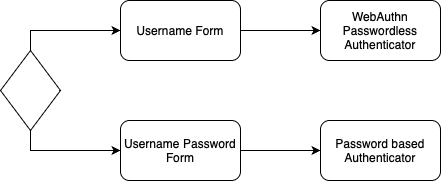
\includegraphics[width=0.7\textwidth]{img/abbildungen/authentication_flow.png}
	\captionsetup{format=hang}
	\caption{Authentication Flow} \label{auth-flow}
\end{figure}

Nach der einer erfolgreichen Konfiguration des Authentication Flows, entstehen zwei neue Prozesse für die Anmeldung und für die Registrierung eines Nutzers. Diese werden in den folgenden Grafiken dargestellt:

\begin{figure}[H]
	\centering 
	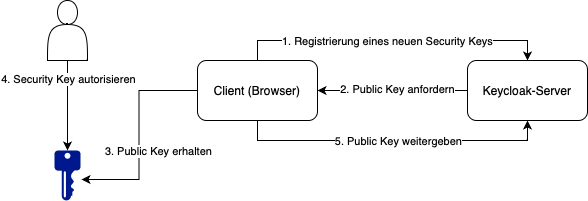
\includegraphics[width=1\textwidth]{img/abbildungen/register_simplified.png}
	\captionsetup{format=hang}
	\caption{Registrierung (vereinfacht)}
\end{figure}

\begin{figure}[H]
	\centering 
	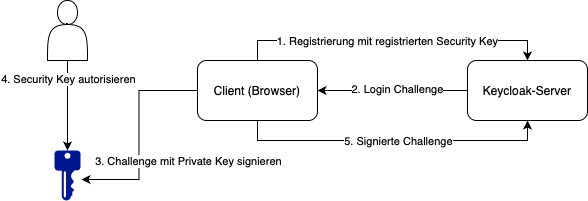
\includegraphics[width=1\textwidth]{img/abbildungen/login_simplified.png}
	\captionsetup{format=hang}
	\caption{Anmeldung (vereinfacht)}
\end{figure}

Die Grafiken stellen den vereinfachten Ablauf der Registrierung und Anmeldung mit Hilfe eines Security Keys dar. Eine detailierte technische Erläuterung und Darstellung der Funktionsweise ist \textbf{\ref{fido2}}zu finden. Der entscheidende Unterschied der beiden Prozesse ist allerdings, dass bei der Registrierung lediglich der öffentliche Schlüssel übergeben wird, während bei der Anmeldung der private Schlüssel benötigt wird. Dieser wird allerdings nicht übergeben, sondern signiert eine Login Challenge, welche vom Keycloak-Server generiert wird. Kann der Keycloak-Server die Signatur mit Hilfe des gespeicherten öffentlichen Schlüssels verifizieren, wird der Nutzer authentifiziert. Sowohl die Registrierung als auch die Anmeldung erfolgen hierbei also nicht über die Anwendung selbst, sondern über den Keycloak-Server und dessen Nutzeroberfläche.

\section{User Feedback}
Um eine Aussage über die Akzeptanz und die Benutzerfreundlichkeit der aufgezeigten Umsetzung zu treffen, wird ein Feedback von den Nutzern der Abteilung cGroup Solutions eingeholt. Um eine wissenschaftliche Aussage zu treffen wird ein Fragebogen erstellt. Es handelt sich dabei um eine Mischform aus einer qualitativen und einer quantitativen Befragung. So wird es ermöglicht eine numerische Auswertung der Antworten zu erhalten, sowie eine qualitative Auswertung der Kommentare. Im Folgenden wird die Durchführung des Fragebogens beschrieben.

\subsection{Rahmen des Feedbacks}
Da zum Zeitpunkt der Erstellung dieser Arbeit die Nutzung keine Umsetzung einer passwortlosen Authentifizierung innerhalb der gesamten \ac{LSY} möglich ist (siehe Kapitel) wird das Feedback auf die Abteilung cGroup Solutions beschränkt. Diese ist zuständig für das in Kapitel beschriebene Produkt cFront, in welchem die passwortlose Authentifizierung testweise implementiert wurde. Die Abteilung besteht aus 15 Personen.

Über einem Zeitraum von zwei Wochen werden alle Mitglieder eingeladen an der Befragung teilzunehmen. Eine Teilnahme ist freiwillig. Die Befragung findet im Büro der Abteilung statt und wird von dem Autor dieser Arbeit durchgeführt. Jeder Teilnehmer wird einzeln und vor Ort befragt. Dies ermöglicht es mit jedem Teilnehmer eine Live-Demonstration durchzuführen. So wird ebenfalls ermöglicht, dass Teilnehmer bereits während der Befragung und der Demonstration Kommentare hinterlassen können. Diese werden auf dem Fragebogen festgehalten und werden für die qualitative Auswertung genutzt werden.

Während der gesamten Demonstration und Befragung werden den Teilnehmern keine Informationen zum Fido2 Protkoll vermittelt, da sonst die Aussagekraft des Feedbacks verfälscht werden könnte. Ziel ist es den ersten Eindruck aller Teilnehmer zu erhalten, ohne dass diese eine erzwungene Einführung in die Thematik erhalten. Die Live-Demonstration beinhaltet die Registrierung und Anmeldung mit Hilfe eines Security Keys, sowie eine Demonstration einer möglichen Anmeldung mit Hilfe eines Passkeys. Zusätzlich erhalten die Teilnehmer die Möglichkeit den Security Key physich zu betrachten. Ein detailierter Verlauf der Demonstartion wird im weiteren Verlauf der Arbeit beschrieben.

\subsection{Auswahl der Teilnehmer}
Zur Durchführung des Fragebogens wurden alle Mitglieder des Teams eingeladen, eine Teilnahme war jedoch freiwillig. Zwei der Mitglieder der Abteilung konnten auf Grund eines Urlaubs nicht an der Befragung teilnehmen. Vor der Durchführung wurden alle Teilnehmer darüber informiert zu welchem Zweck die Daten für diese Arbeit erhoben werden. Die Befragung stand dabei nicht anonym statt, um einen Austausch zwischen dem Autor und den Teilnehmern zu ermöglichen. Da die Befragung die Abteilung der Teilnehmer betrifft sollten diese somit eine Möglichkeit bekommen, ihre Gedanken zu dem modifiziertem Anmeldevorgang zu teilen.

14 Mitglieder der Abteilung stimmten der Teilnahme an der Befragung zu. Die letzte Person befand sich während des möglichen Zeitraumes der Befragung im Urlaub. Das durchschnittsalter der Teilnehmer beträgt 45,4 Jahre. Die genaue Verteilung wird in der folgenden Grafik sichtbar:

\begin{figure}[h]
	\centering 
	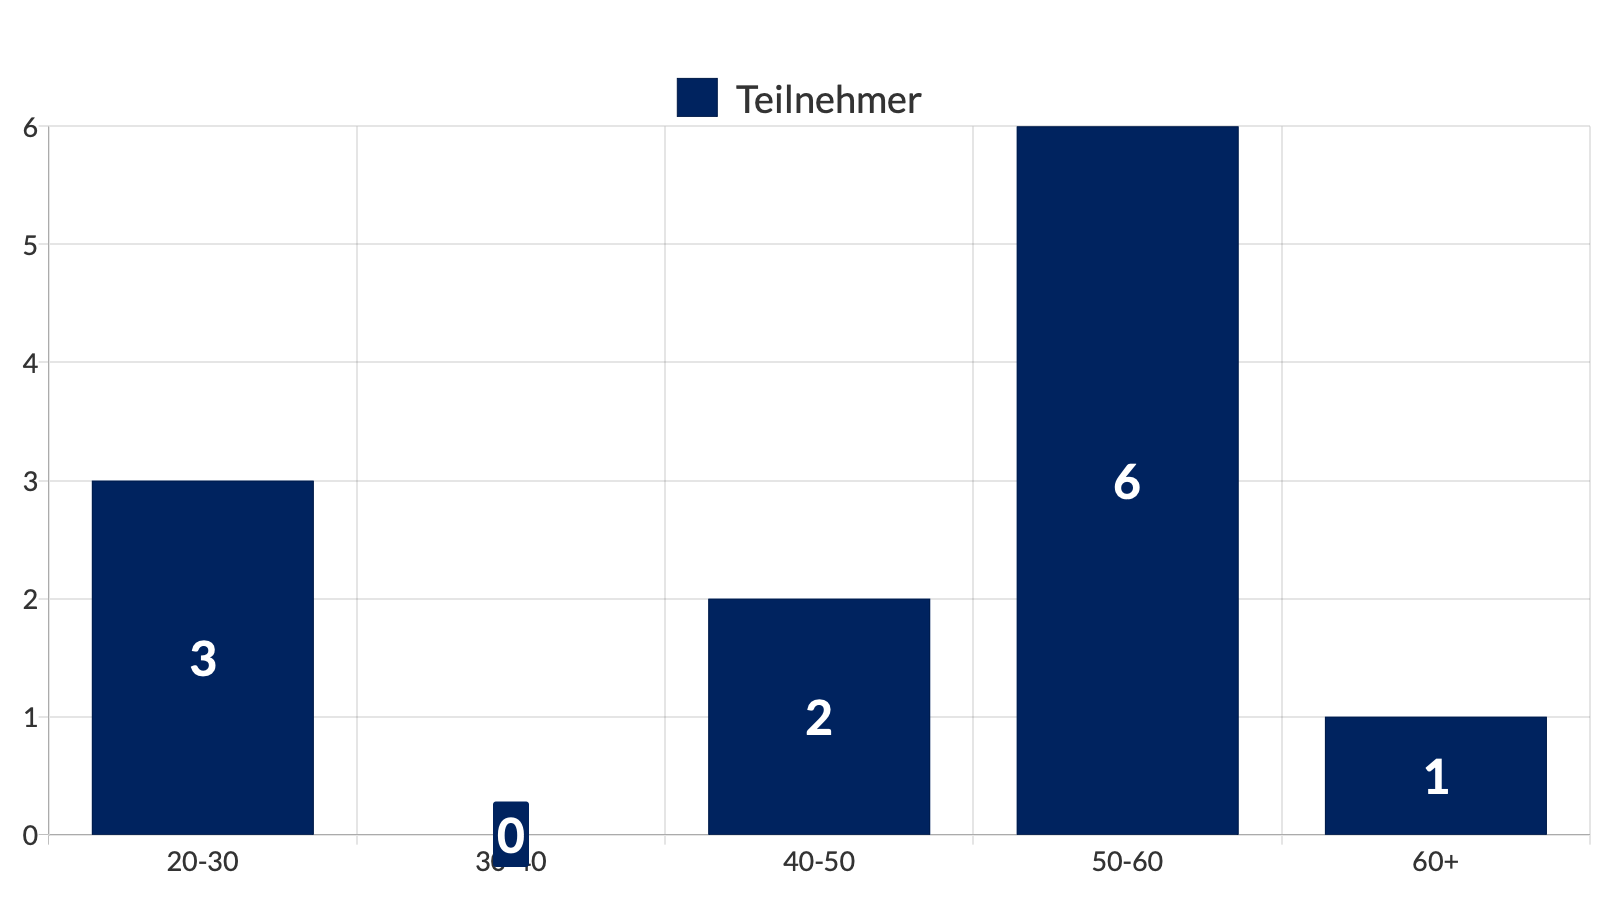
\includegraphics[width=0.8\textwidth]{img/abbildungen/chart-2.png}
	\captionsetup{format=hang}
	\caption{Alter der Teilnehmer}
\end{figure}

Dabei ist auffällig, dass die Teilnehmer der Befragung überwiegend der Gruppe 50-60 Jahre zugehörig sind. Auch die Gruppe 20-30 Jahre ist häufig vertreten. Lediglich die Gruppe 40-50 Jahre ist wenig vertreten. Daraus lässt sich schließen, dass die Teilnehmer der Befragung überwiegend entweder neu in das Berufsfeld eingestiegen sind oder bereits eine langjährige Erfahrung in diesem Bereich haben. 

Vor Beginn der Befragung wurden die Teilnehmer gebeten anzugeben, welche Rolle sie innerhalb des Teams einnehmen. Daraus lassen sich zwei Gruppen bilden: Development und Operations. Die Verteilung der Teilnehmer auf die beiden Gruppen ist in der folgenden Grafik dargestellt:

\begin{figure}[h]
	\centering 
	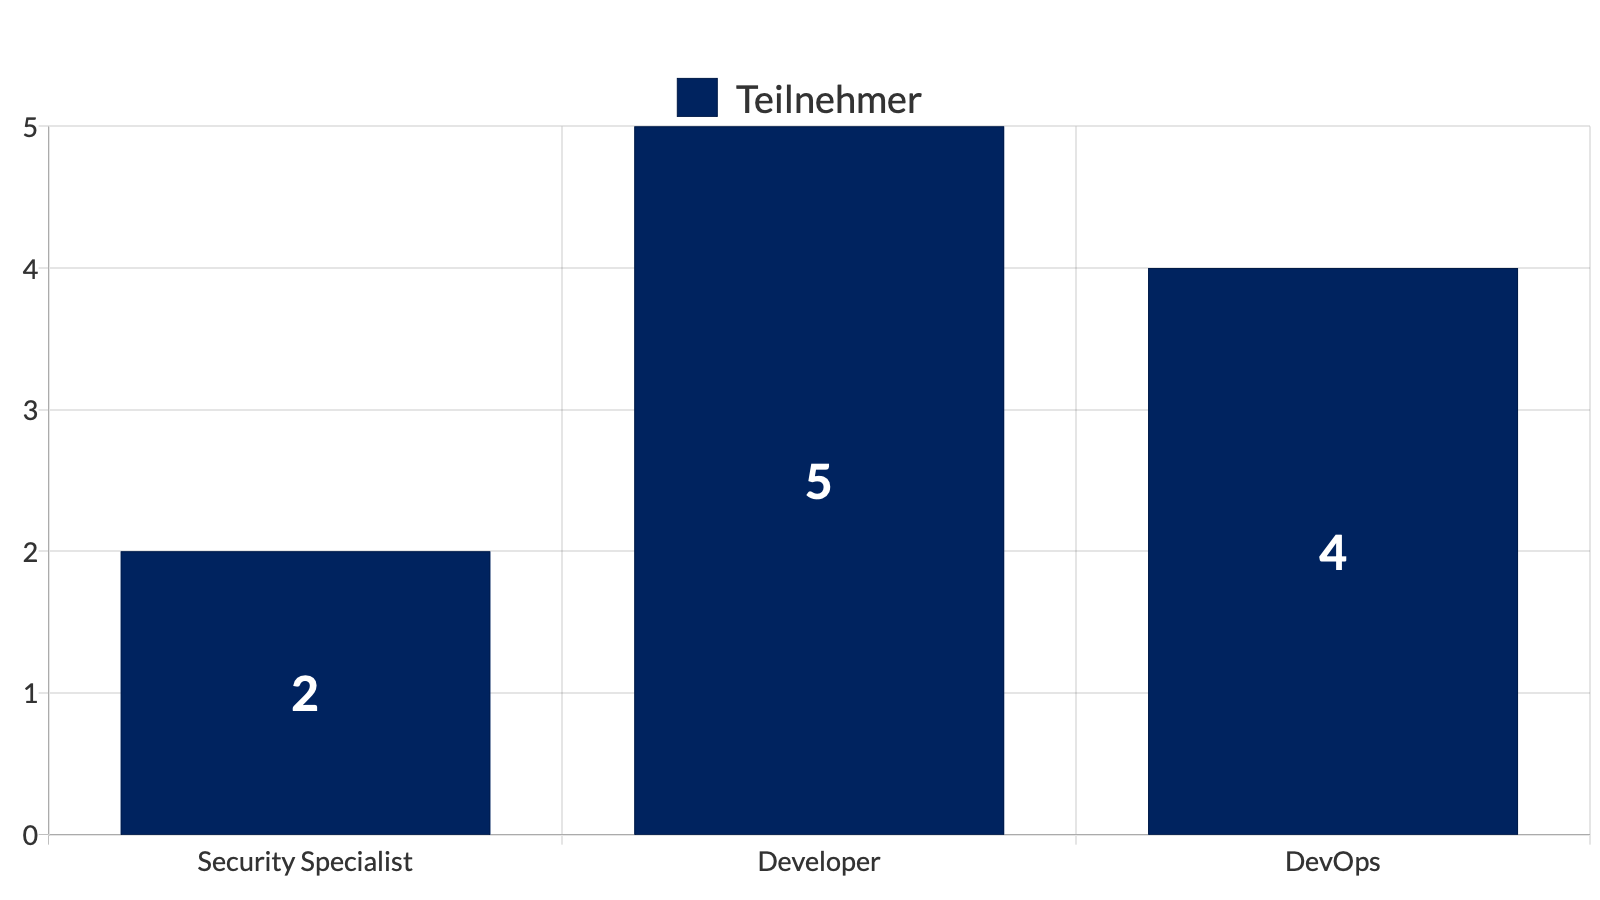
\includegraphics[width=0.7\textwidth]{img/abbildungen/chart_rollen.png}
	\captionsetup{format=hang}
	\caption{Alter der Teilnehmer}
\end{figure}

\subsection{Inhalt der Demonstration}
Allen Teilnehmern wurde vor der Befragung eine Live-Demonstration der Registrierung und Anmeldung mit Hilfe eines Security Keys gezeigt. Der Security Key wurde zu Beginn der Demonstration in einen üblichen USB-Slot eines Firmenlaptops eingesteckt und nach der Demonstration an die Teilnehmer übergeben. 

Die Anmeldung/Registrierung ist in mehrere Schritte unterteilt. Zunächst bestätigt der Nutzer, dass er sich mit Hilfe eines Security Keys anmelden/registrieren möchte:

\begin{figure}[h]
	\centering 
	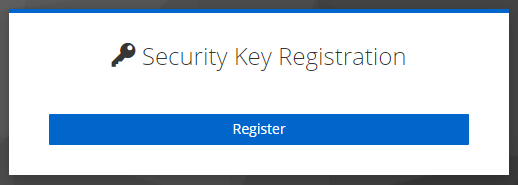
\includegraphics[width=0.7\textwidth]{img/abbildungen/reg001.png}
	\captionsetup{format=hang}
	\caption{Veränderter Keycloak-Login}
\end{figure}

Darauf folgt ein Dialogfeld des Browsers, welcher den Nutzer dazu auffordert zu bestätigen, dass der Security Key registriert wird. Dieser Schritt ist einmalig und findet nur bei der Registrierung statt. Ist der Security Key bereits registriert, wird dieser Schritt übersprungen:

\begin{figure}[h]
	\centering 
	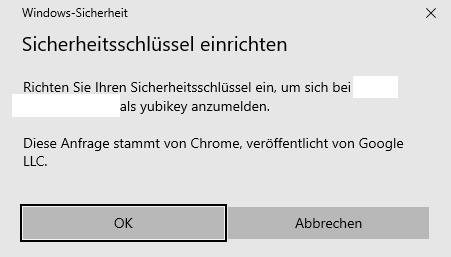
\includegraphics[width=0.7\textwidth]{img/abbildungen/reg002.png}
	\captionsetup{format=hang}
	\caption{Veränderter Keycloak-Login}
\end{figure}

Nach der Bestätigung des Dialogs muss der Nutzer den PIN des Security Keys eingeben:

\begin{figure}[H]
	\centering 
	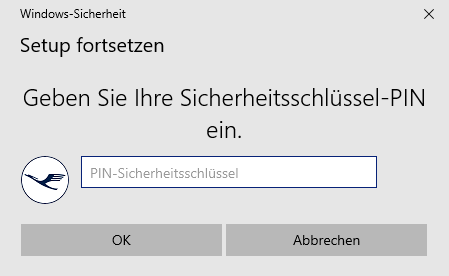
\includegraphics[width=0.7\textwidth]{img/abbildungen/reg003.png}
	\captionsetup{format=hang}
	\caption{Veränderter Keycloak-Login}
\end{figure}

Ist die richtige PIN eingegeben wurden, erscheint ein letztes Fenster, welches den Nutzer dazu auffordert den Knopf des Security Keys zu drücken. Erst danach ist der Browser dazu autorisert sich mit Hilfe des Security Keys gegen den Keycloak-Server zu registrieren oder anzumelden:

\begin{figure}[h]
	\centering 
	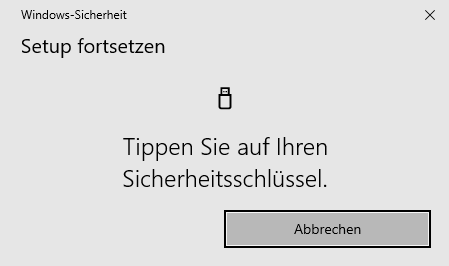
\includegraphics[width=0.7\textwidth]{img/abbildungen/reg004.png}
	\captionsetup{format=hang}
	\caption{Veränderter Keycloak-Login}
\end{figure}

Sobald der Knopfdruck erfolgt, wird der Nutzer erfolgreich eingeloggt. Diese Informationen wurden den Teilnehmern ebenfalls während der Durchführung des Fragebogens mitgeteilt. 

Nachdem die Registrierung und Anmeldung mit Hilfe eines Security Keys demonstriert wurde, wurde den Teilnehmern ebenfalls eine mögliche Anmeldung mit Hilfe eines Passkeys gezeigt. Der Prozess beginnt ebenfalls bei Abbildung xy und hat lediglich einen Folgeschritt:

\begin{figure}[h]
	\centering 
	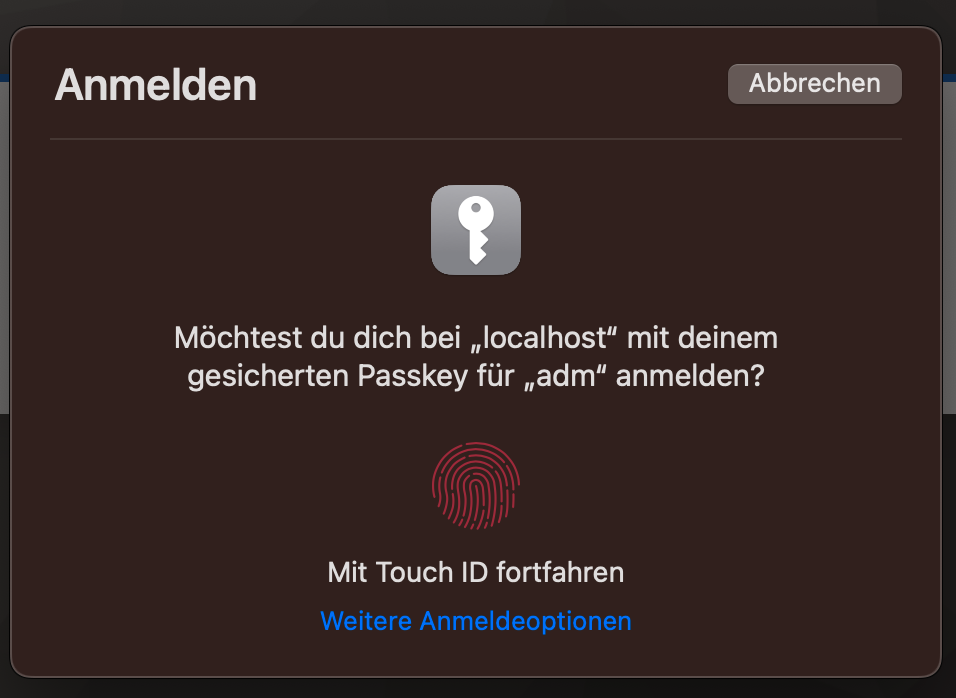
\includegraphics[width=0.7\textwidth]{img/abbildungen/passkey_demo.png}
	\captionsetup{format=hang}
	\caption{Veränderter Keycloak-Login}
\end{figure}

Für die Demonstration wurde hierbei ein privates Gerät genutzt (Apple Macbook Air M1), welches mit einem Touch ID Scanner ausgestattet ist.


\subsection{Herleitung der Fragen} \label{questions}
Aufgrund des Ziels der Befragung, eine Aussage über die Akzeptanz und die Benutzerfreundlichkeit einer passwortlosen Authentifizierung zu treffen, werden lediglich Fragen gestellt, die sich auf diese beiden Punkte beziehen. Um eine hohe Teilnahme zu gewährleisten, werden die Fragen möglichst kurz gehalten und nur wenige Fragen gestellt. Die Fragen werden so gestaltet, dass sie dem Teilnehmer die Möglichkeit bietet Kommentare zu hinterlassen oder seine Antwort zu begründen. Die Fragen werden so gestellt, dass sie einfach zu verstehen sind und kein Vorkenntnisse im Bereich der passwortlosen Authentifizierung voraussetzen. Im folgenden werden die Fragen begründet aufgelistet und erläutert:

\paragraph{Frage 1:}

\begin{quote}
    \textit{Hast du schonmal einen Security Key genutzt?}
\end{quote}
\textbf{Antwörtmöglichkeiten:} Ja; Nein; 

Diese Frage leitet sich aus \cite{farke2020you} ab. Die Antwortmöglichkeiten werden im Vergleich aber angepasst und reduziert. Durch die Reduzierung auf zwei Antwortmöglichkeiten wird eine bessere Auswertung ermöglicht. Antworten Teilnehmer mit \textit{Ja}, werden sie gefragt in welchem Kontext sie den Security Key genutzt haben. So lassen sich zusätzliche Informationen über die Nutzungsdauer und den Zweck der Nutzung zu erhalten.

\paragraph{Frage 2:}

\begin{quote}
    \textit{Bist du generell bereit deine Passwörter durch eine andere Art der Authentifizierung zu ersetzen?}
\end{quote}
\textbf{Antwörtmöglichkeiten:} Ja; Nein; 

Diese Frage ergibt sich aus einer Umfrage von Statista, in welcher Teilnehmer gefragt wurden, durch welche Art der Authentifizierung sie das Passwort ersetzen würden. Lediglich 22\% der Teilnehmer gaben an, dass sie ihr Passwort lieber beibehalten würden \cite{techstat}. Daraus folgt die Annahme, dass eine Vielzahl an Nutzern grundsätzlich dazu bereit wären ihr Passwort zu ersetzen. Die Frage soll eine bessere Analyse der folgenden Fragen ermöglichen und zielt auf die Akzeptanz einer passwortlosen Authentifizierung im generellen ab.

\paragraph{Frage 3:}

\begin{quote}
    \textit{Benutzt du auf der Arbeit aktuell einen Passwort Manager?}
\end{quote}

\textbf{Antwörtmöglichkeiten:} Ja; Nein;

Verwandte Studien zeigen, dass Nutzer eines Passwort Managers teilweise eine geringere Anmeldezeit auf Grund eines Passwort Managers aufweisen (insbesondere bei einer Nutzung von autofill) \cite{farke2020you}. Die Frage soll einen Zusammenhang zwischen der Nutzung eines Passwort Managers und der Einschätzung der Benutzerfreundlichkeit einer passwortlosen Authentifizierung ermöglichen.

\paragraph{Frage 4:}

\begin{quote}
    \textit{Kennst du das FIDO2-Protokoll und weißt du grob wie es funktioniert?}
\end{quote}

\textbf{Antwörtmöglichkeiten:} Ja; Nein;

Diese Frage bezieht sich auf die in Kapitel xy aufgeführte Problematik, dass Nutzer lieber Passwörter nutzen, da sie die Funktionsweise und Technologie im Hintergrund besser verstehen. Dieser mögliche Zusammenhang soll betrachtet werden. Antworten Teilnehmer mit \textit{Ja}, werden sie gefragt, ob sie die Funktionsweise des FIDO2-Protokolls erklären können. So lässt sich eine Aussage über die Kenntnisse der Teilnehmer treffen. 

\paragraph{Frage 5:}

\begin{quote}
    \textit{Wie bewertest du die Benutzerfreundlichkeit der Registrierung mit Hilfe eines Security Keys?}
\end{quote}

\textbf{Antwörtmöglichkeiten:} Besser als mit einem Passwort; Gleich gut wie mit einem Passwort; Schlechter als mit einem Passwort;

Diese Frage soll einen Vergleich zwischen der Benutzerfreundlichkeit einer passwortlosen Authentifizierung und einer passwortbasierten Authentifizierung ermöglichen. Aus diesem Grund wurden die Antwortmöglichkeiten bewusst so gewählt, dass sie einen Vergleich ermöglichen. Eine generelle Bewertung würde die Auswertung erschweren, da die Teilnehmer unterschiedliche Vergleichswerte wählen könnten.

\paragraph{Frage 6:}

\begin{quote}
    \textit{Wie bewertest du die Benutzerfreundlichkeit der Anmeldung mit Hilfe eines Security Keys?}
\end{quote}

\textbf{Antwörtmöglichkeiten:} Besser als mit einem Passwort und \ac{MFA}; Gleich gut wie mit einem Passwort und \ac{MFA}; Schlechter als mit einem Passwort und \ac{MFA};

Wie auch Frage fünf zielt diese Frage auf die Benutzerfreundlichkeit ab. Die Unterteilung in zwei Fragen ergibt sich vor allem aus der Tatsache, dass sich die Registrierung und die Anmeldung, insbesondere bei einer passwortbasierten Authentifizierung, deutlich unterscheiden. Während es sich bei einer Anmeldung lediglich um eine Wissensabfrage handelt, muss bei der Registrierung zunächst ein eigenes Passwort erstellt werden. Dies könnte dazu führen, dass die beiden Abläufe unterschiedlich bewertet werden und somit der Vergleich zur passwortlosen Authentifizierung erschwert wird.

\paragraph{Frage 7:}

\begin{quote}
    \textit{Wärst du dazu bereit einen Security Key für den privaten Gebrauch zu kaufen, wenn der Preis bei ca. 50€ liegt?}
\end{quote}

\textbf{Antwörtmöglichkeiten:} Ja; Nein;

Diese Frage zielt auf die Akzeptanz einer passwortlosen Authentifizierung im privaten Kontext ab und basiert auf dem Ergebnis aus Kapitel xy. Dort wurde festegestellt, dass der Kaufpreis eines Security Keys ebenfalls eine Hürde für die Nutzung darstellen kann. Als Richtwert für den Kaufpreis wird hierbei der ungefähre Preis eines Yubikeys der Series 5 mit NFC gewählt, da dieser ebenfalls für die Umsetzung genutzt wird. Die Frage soll im Weiteren auch auf für die Nutzung im Unternehmenskontext genutzt werden, da die Akzeptanz im Generellen auch eine Auswirkung auf die Etablierung von Security Keys hat. Eine erhöhte Etablierung kann ebenfalls zu einer breiteren Unterstüzung führen.

\paragraph{Frage 8:}

\begin{quote}
    \textit{Hältst du einen Security Key für sicherer als ein Passwort?}
\end{quote}

\textbf{Antwörtmöglichkeiten:} Ja; Nein;

Diese Frage basiert auf der in Kapitel xy beschriebenen Annahme, dass Nutzer an der Sicherheit von Security Keys zweifeln, da sie die Funktionsweise der Technologie nicht verstehen. Dies soll im Zusammenhang mit Frage 4 betrachtet werden. Bewusst wird dabei auf die Antwortmöglichkeit \textit{Ich weiß es nicht} verzichtet, da Teilnehmer auf der Basis ihres aktuellen Wissensstands eine intuitive Entscheidung treffen sollen. Dies ermöglicht ebenfalls eine Aussage über die Akzeptanz der Teilnehmer. 

\paragraph{Frage 9:}

\begin{quote}
    \textit{Findest du eine Anmeldung per Passkey besser als eine Anmeldung per Security Key?}
\end{quote}

\textbf{Antwörtmöglichkeiten:} Ja; Nein; Gleich;

Diese Frage soll für einen Ausblick genutzt werden, ob eine Anmeldung per Passkey eine Alternative zu einer Anmeldung per Security Key darstellt. In \textbf{\ref{fido2-pros}} wurde ebenfalls deutlich, dass die Benutzerfreundlichkeit weniger von \ac{FIDO}2 abhängig ist, sondern viel mehr vom genutzten authentifizerungsgerät.  Mit Hilfe von kommentaren der Teilnehmer sollen konkrete Vor- und Nachteile der beiden Verfahren in Bezug auf deren Benutzerfreundlichkleit ermittelt werden.


\subsection{Auswertung}
Die Auswertung der Fragebögen bestätigt in vielen Teilen die bereits erarbeiteten Annahmen aus Kapitel xy. Lediglich zwei der Teilnehmer geben an, dass sie bereits einen Security Key genutzt haben. Dies allerdings nur testweise und nicht im alltäglichen Gebrauch. Die restlichen Teilnehmer geben an, dass sie noch keinen Security Key genutzt haben bzw. lediglich einen gesehen haben. Dies bestätigt, dass die Nutzung von Security Keys aktuell noch nicht weit verbreitet ist und Passwörter weiterhin die dominierende Methode der Authentifizierung darstellen.

Alle Teilnehmer geben an, dass sie dazu bereit wären ihr Passwort durch eine andere Art der Authentifizierung zu ersetzen. Dies übertrifft das Ergebnis aus \cite{techstat}. Dies kann daran liegen, dass alle Teilnehmer in einem sehr technischen Kontext arbeiten und somit eine höhere Akzeptanz für neue Technologien aufweisen und ein höheres Bewusstsein für Sicherheit innerhalb der Informatik aufweisen. 

\begin{figure}[H]
	\centering 
	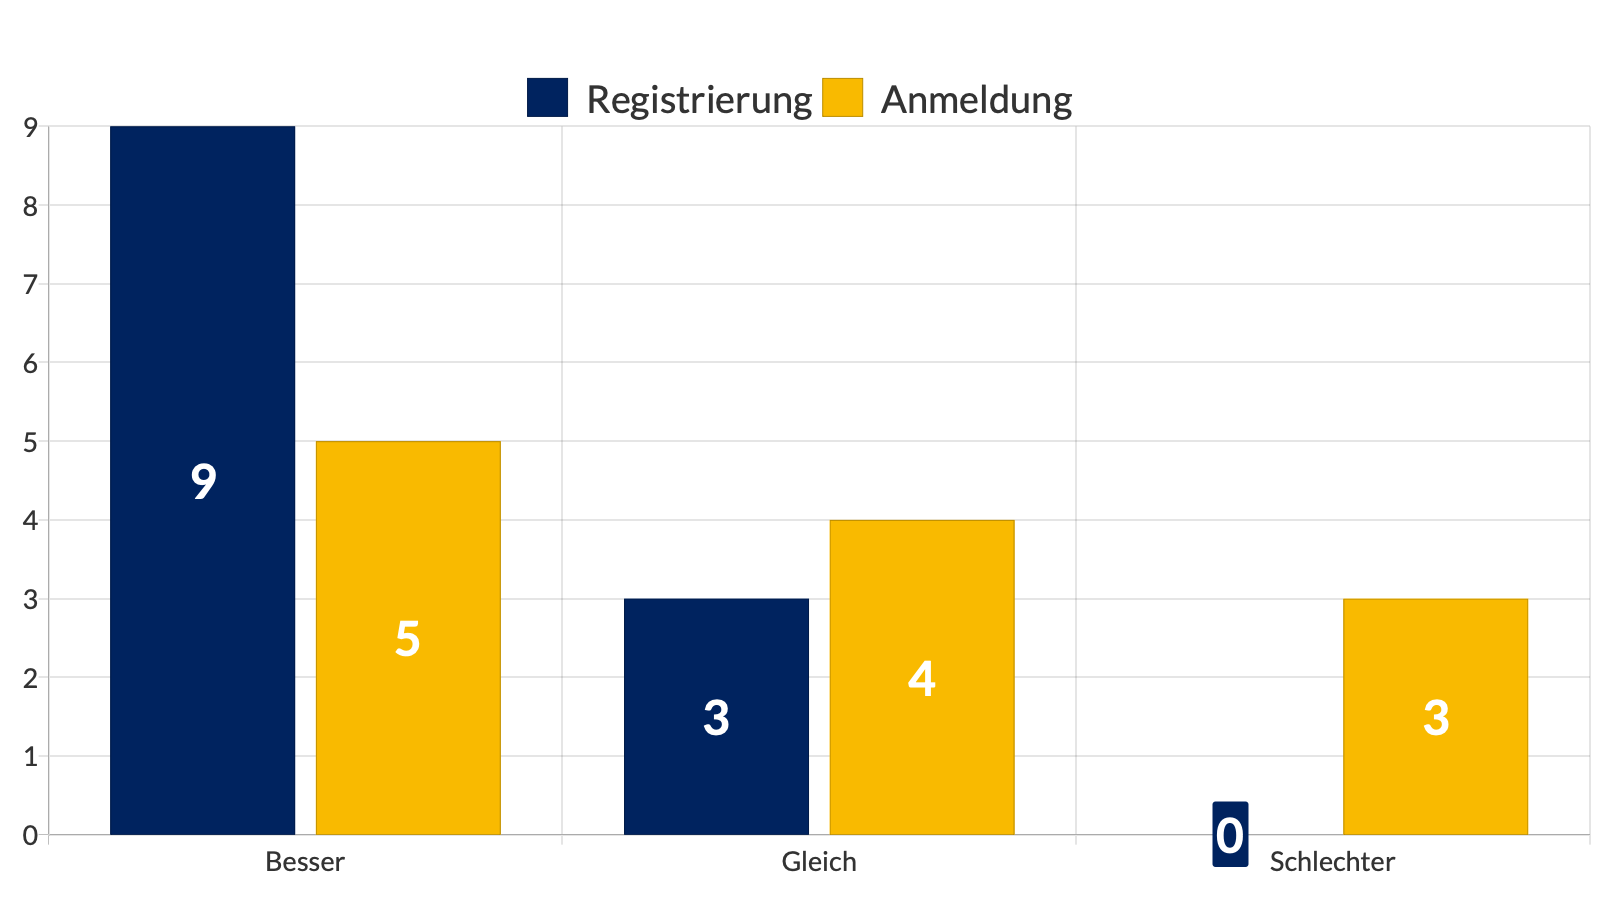
\includegraphics[width=0.7\textwidth]{img/abbildungen/chart_anmeldung_register.png}
	\captionsetup{format=hang}
	\caption{Veränderter Keycloak-Login}
\end{figure}

Bei der Bewertung der Registrierung und der Anmeldung mit Hilfe eine Security Keys sind deutliche Unterschiede sichtbar. Die deutliche Mehrheit der Teilnehmer bevorzugte die Registrierung per Security Key gegenüber der passwortbasierten Alternative. Keiner der Teilnehmer fand die Registrierung im Vergleich schlechter. Bei der Anmeldung hingegen ist ein ausgeglicheneres Ergebnis sichtbar. Im Vergleich geben drei der Teilnehmer an, dass sie Anmeldung schlechter finden als die aktuelle Alternative mit Hilfe eines Passwortes und \ac{MFA}. Es wird also deutlich, dass die beiden Abläufe der Registrierung und der Anmeldung differenziert betrachtet werden müssen. 
Eine Abhängigheit zwischen der Nutzung eines Passwort Managers und der Bewertung der Benutzerfreundlichkeit lässt sich nicht feststellen, da lediglich drei Teilnehmer keinen Passwort Manager nutzen und diese sehr verschiedene Bewertungen abgeben. Eine aussagekräftige Auswertung ist somit nicht möglich. 


Zehn der Teilnehmen geben an, dass sie nicht bereit wären 50€ für einen Security Key auszugeben. Dies bestätigt die Annahme aus Kapitel xy, dass der Preis eine Hürde für die Nutzung und Etablierung darstellen kann. Eine vermehrte Nutzung im privaten Kontext würde zu mehr Akzeptanz führen, da die Teilnehmer bereits mit der Technologie vertraut sind. 

Bis auf zwei Teilnehmer wird die Nutzung von Security Keys sicherer eingeschätzt als die Nutzung von Passwörtern. Da lediglich zwei Nutzer die Nutzung als weniger sicher betrachten lässt sich keine Aussage über einen Zusammenhang zwischen der Kenntnis des FIDO2-Protokolls und der Einschätzung der Sicherheit treffen.

Zwölf der Teilnehmer geben an eine Anmeldung per Passkey besser zu finden als eine Anmeldung per Security Key. 

Aus den Kommentaren lassen sich ebenfalls einige Erkenntnisse ziehen:

\begin{itemize}
    \item Ein Teilnehmer stufte die Registrierung und ANmeldung als \glqq\textit{sehr aufregend}\grqq, da es etwas neues ist und begründete so seine positive Bewertung. Dieses Beispiel zeigt auf, dass die Gewöhnung an eine neue Technologie nicht zwangsweise negativ ist, sondern auch positiv bewertet werden kann.
    \item Mehrere Teilnehmer kritisierten die Notwendigkeit den Security Key immer dabei haben zu müssen und spontane Logins nicht möglich sind. Dies deckt sich mit den Ergebnissen aus Kapitel xy.
    \item Daraus resultiere auch der Kritikpunkt, dass zusätzliche Hardware verloren gehen kann. Dies ist ein weiterer Kritikpunkt, welcher bereits in Kapitel xy aufgeführt wurde.
    \item Mehrere Teilnehmer wiesen darauf hin, dass sie ihr Handy und somit ihre Authenticator App im dabei haben. Selbst, wenn sie den Prozess des anmeldens mit Hilfe eines Security Keys als besser bewerten, würden sie weiterhin die Nutzung eines Passwortes mit \ac{MFA} bevorzugen. 
    \item Ein neuer Punkt der in den Kommentaren aufgeführt wurde ist, dass \ac{SSO} ein wichtiger Faktor ist. Da somit eine geringere Abfrage der Passwörter gegeben ist und auch weniger Passwörter erstellt werden müssen. Dies wirkt sich auch auf die EInschätzung der Benutzerfreundlichkeit aus.
    \item Die Mehrheit der Teilnehmer war der Meinung, dass sie die Benutzerfreundlichkeit der Security Keys erst nach einer längeren Testphase bewerten können.
    \item Ein Kritikpunkt der Teilnehmer am Anmeldevorgang mit Hilfe eines Security Keys ist, dass die EIngabe der PIN und des Benutzernamens zu viel sind. Dadurch bewerteten sie die Alternative als gleich oder schlechter als die aktuelle Lösung. Sie wünschen sich eine Lösung, bei dem der Security Key lediglich eingesteckt und gedrückt werden muss.
    \item Ein Teilnehmer begründete seine Antwort bezogen auf die Passkeys damit, dass er zusätzliche Hardware für sicherer hält und sich bei der Nutzung von Passkeys nicht sicher ist, ob diese wirklich nur auf dem Gerät gespeichert werden.
    \item Einige Teilnehmer erläuterten, dass sie die Anmeldung per Security Key benutzerfreundlicher als ein Passwort mit \ac{MFA} finden, allerdings nicht besser als lediglich einem Passwort.
    \item Ebenfalls wurde die mechanische Belastung des Security Keys und des USB-Ports genannt. Beide könnten durch die Nutzung beschädigt werden. Auch dieser Punkt wurde bereits in Kapitel xy aufgeführt.
    \item Auch der Preis wurde häufig als Kritikpunkt genannt. Ergänzend erwähnte allerdings ein Teilnehmer, dass er den Preis bezahlen würde, wenn es weiter etabliert ist. Ein anderer Teilnehmer erwähnte, dass er zum aktuellen Zeitpunkt maximal 20€ für einen Security Key ausgeben würde.
    \item Zur reinen Benutzerfreundlichkeit merkte ein Teilnehmer an, dass ein schlechtes und einfach gewähltes Passwort deutlich benutzerfreundlicher sei, wenn man den Faktor der Sicherheit nicht betrachtet.
\end{itemize}

\subsection{Fazit \& Reflexion}
Aus der Auswertung der Kommentare lässt sich ebenfalls eine Reflexion des Fragebogens ableiten. Ein entscheidenes Feedback ist dabei, die Testphase zu verlängern. Da der Bearbeitungszeitraum dieser Arbeit begrenzt ist und zunächst eine Implementierung erfolgen musste war dies nicht möglich. Aus diesem Grund wurde lediglich dieser Fragebogen erstellt, um einen ersten Eindruck zu erhalten. Für eine weitere Ausarbeitung sollte allerdings eine längere Testphase eingeplant werden. 


\section{Wirtschaftlichkeit}
Ein entscheidender Faktor für den Einsatz einer passwortlosen Authentifizierung mit Hilfe eines Security Keys ist die Wirtschaftlichkeit. Im Folgenden soll eine Analyse der Wirtschaftlichkeit im Bezug auf die Abteilung cGroup Solutions durchgeführt werden.

Betrachtet man die Teamgröße von 15 Personen und geht von den aktuellen Kosten eines Yubikeys aus (50€) so ergibt sich ein Gesamtpreis von 750€. Dieser Preis ist einmalig und muss nicht wiederholt werden. Auf Grund der geringen Backup-Möglichkeiten eines Security Keys sollte allerdings ein Backup-Key pro Nutzer angeschafft werden. Dieser kann im Falle eines Verlustes des ersten Keys genutzt werden. Dies erhöht die Kosten auf 1500€.
Lässt man alternativ weiterhin eine Anmeldung per Passwort zu, würden 750€ entfallen, allerdings wäre der eigentliche Zweck der Anschaffung nicht mehr erfüllt.
Sollte ein Security Key verloren oder kaputt gehen muss dieser ebenfalls ersetzt werden.
Zusätzlich zu den Materialkosten müssen die Kosten für die Implementierung betrachtet werden. Die Migration von Passwörtern auf Security Keys muss von erfahrenen Entwicklern und Architekten durchgeführt werden. Die genauen Kosten dafür lassen sich allerdings nicht definieren und sind stark abhängig von der gewünschten Implementierung. 

Sollte eine Anschaffung für das gesamte Unternehmen \ac{LSY} erfolgen so würde sich der Preis auf 280.000€ belaufen. Dies ergibt sich aus der aktuellen Mitarbeiterzahl von 2.800€ und den Kosten eines Security Keys von 50€, sowie einem Backup-Key pro Nutzer.

Im Gegenzug muss ein möglicher Kostenvorteil eingerechnet werden. Da Passwörter wie in Kapitel xy beschrieben eine der größten Schwachstellen darstellen, sind sie ein grundlegender Faktor für erfolgreiche Angriffe. Würde eine Nutzung der Security Keys dies verhindern oder eindämmen, so würde dies zu einer Kostenreduktion führen. Auch hier lassen sich allerdings nur schwierig konkrete Zahlen nennen. Diese sind unter anderem abhängig von der Schwere und Art des Angriffs. Einen Richtwert liefert der \textit{Cost of a Data Breach Report 2023} von IBM \cite{databreach}. Dort werden die durchschnittlichen Kosten eines Data Breach für bestimmte Regionen aufgezählt. Der Wert für die Region Deutschland liegt bei 4,67 Millionen US-Dollar \cite{databreach}. Daraus lässt sich folgern, dass ein erfolgreicher Angriff auf die \ac{LSY} zu einem deutlich höheren Kostenaufwand führen kann, als die Anschaffung von Security Keys.
